\documentclass[aspectratio=169,12pt,t]{beamer}

% --- Theme: Metropolis (modern, clean) ---
\usetheme[progressbar=frametitle,numbering=fraction,block=fill]{metropolis}

% --- Fira Sans font (install texlive-fonts-extra if missing) ---
\IfFileExists{FiraSans.sty}{\usepackage[sfdefault]{FiraSans}}{}

% --- Light background with warm accent ---
\definecolor{mDarkTeal}{RGB}{35,55,59}
\definecolor{mLightBrown}{RGB}{235,228,216}
\definecolor{mAccent}{RGB}{140,70,20}

\setbeamercolor{normal text}{fg=mDarkTeal,bg=white}
\setbeamercolor{alerted text}{fg=mAccent}
\setbeamercolor{frametitle}{bg=mDarkTeal,fg=white}
\setbeamercolor{progress bar}{fg=mAccent,bg=mLightBrown}
\setbeamercolor{title separator}{fg=mAccent}
\setbeamercolor{progress bar in head/foot}{fg=mAccent,bg=mLightBrown}
\setbeamercolor{progress bar in section page}{fg=mAccent,bg=mLightBrown}

% --- Packages ---
\usepackage[utf8]{inputenc}
\usepackage{amsmath,amssymb,amsthm}
\usepackage{mathrsfs}
\usepackage{tikz}
\usetikzlibrary{arrows.meta,positioning,calc,decorations.pathreplacing,shapes,patterns}
\usepackage{pgfplots}
\pgfplotsset{compat=1.18}
\usepgfplotslibrary{fillbetween}

% --- TikZ diagram styles (shared across the series) ---
\tikzset{
  axisln/.style={-{Stealth[length=2.6mm]}, line width=0.8pt, gray!75},
  curveln/.style={line width=1.6pt, line cap=round, line join=round},
  projln/.style={dash pattern=on 2.6pt off 2pt, line width=0.7pt},
  guide/.style={-{Stealth[length=2.6mm,width=2.2mm]}, line width=1.1pt},
  box/.style={draw=#1, fill=#1!12, line width=1pt, rounded corners=2pt,
    minimum width=5.6cm, minimum height=1.35cm, align=center, font=\small},
}
% point marker with a white halo: \dotpt{color}{(coord)}
\newcommand{\dotpt}[2]{%
  \fill[white] #2 circle (3.6pt);
  \fill[#1] #2 circle (2.4pt);
}
% open point marker: \opendotpt{color}{(coord)}
\newcommand{\opendotpt}[2]{%
  \fill[white] #2 circle (3.6pt);
  \draw[#1, line width=1pt] #2 circle (2.4pt);
}

% --- Semi-transparent white highlight for text on top of background images ---
\usepackage[most]{tcolorbox}

% Inline highlight: \hl{short text}
\newtcbox{\hl}{%
  nobeforeafter, tcbox raise base,
  colback=white, opacityback=0.6,
  colframe=white, opacityframe=0,
  sharp corners, boxsep=2pt, left=3pt, right=3pt, top=2pt, bottom=2pt%
}

% Block highlight: \begin{hlbox} ... \end{hlbox}  (multi-line, paragraphs, itemize)
% Optional argument accepts any tcolorbox key, e.g. [width=0.6\linewidth]
\newtcolorbox{hlbox}[1][]{%
  enhanced, breakable,
  colback=white, opacityback=0.6,
  colframe=white, opacityframe=0,
  boxsep=3pt, left=6pt, right=6pt, top=4pt, bottom=4pt,
  sharp corners,
  {#1}%
}

% --- Custom colors for content types ---
\definecolor{defcolor}{RGB}{25,85,120}
\definecolor{thmcolor}{RGB}{140,35,35}
\definecolor{proofcolor}{RGB}{35,100,50}
\definecolor{excolor}{RGB}{140,75,10}
\definecolor{remcolor}{RGB}{90,90,90}

% --- Beamer blocks for mathematical content types (semi-transparent) ---
\tcbset{hlblockbase/.style={
  enhanced, breakable,
  coltitle=white, fonttitle=\bfseries,
  opacitybacktitle=0.8, opacityback=0.6,
  opacityframe=0,
  sharp corners,
  boxsep=1pt, left=5pt, right=5pt, top=2pt, bottom=2pt,
  toptitle=1pt, bottomtitle=1pt,
  before upper={\setlength{\abovedisplayskip}{4pt}\setlength{\belowdisplayskip}{4pt}}
}}

\newtcolorbox{defblock}[1]{hlblockbase, title={#1},
  colbacktitle=defcolor, colback=defcolor!15, colframe=defcolor}
\newtcolorbox{thmblock}[1]{hlblockbase, title={#1},
  colbacktitle=thmcolor, colback=thmcolor!15, colframe=thmcolor}
\newtcolorbox{proofblock}[1]{hlblockbase, title={#1},
  colbacktitle=proofcolor, colback=proofcolor!15, colframe=proofcolor}
\newtcolorbox{exblock}[1]{hlblockbase, title={#1},
  colbacktitle=excolor, colback=excolor!15, colframe=excolor}
\newtcolorbox{remblock}[1]{hlblockbase, title={#1},
  colbacktitle=remcolor, colback=remcolor!15, colframe=remcolor}

% --- Metadata ---
\title{Chapter 7: Sequences and Series of Functions}
\subtitle{Section: Uniform Convergence and Integration}
\author{Based on Walter Rudin's \emph{Principles of Mathematical Analysis}}
\date{}

% --- Shared plot helpers for this deck ---
% Example 7.6 (second version): g_n(x) = n x (1 - x^2)^n, integral n/(2n+2)
\pgfmathdeclarefunction{bump}{2}{\pgfmathparse{(#2)*(#1)*(1-(#1)^2)^(#2)}}
% Tube picture: f_n and a wiggly f within eps of f_n
\pgfmathdeclarefunction{tubefn}{1}{\pgfmathparse{2.2+0.8*sin(deg(0.9*(#1)))+0.12*(#1)}}
\pgfmathdeclarefunction{tubef}{1}{\pgfmathparse{2.2+0.8*sin(deg(0.9*(#1)))+0.12*(#1)+0.3*sin(deg(5*(#1)))*cos(deg(2.3*(#1)))}}

\begin{document}

{
\usebackgroundtemplate{%
  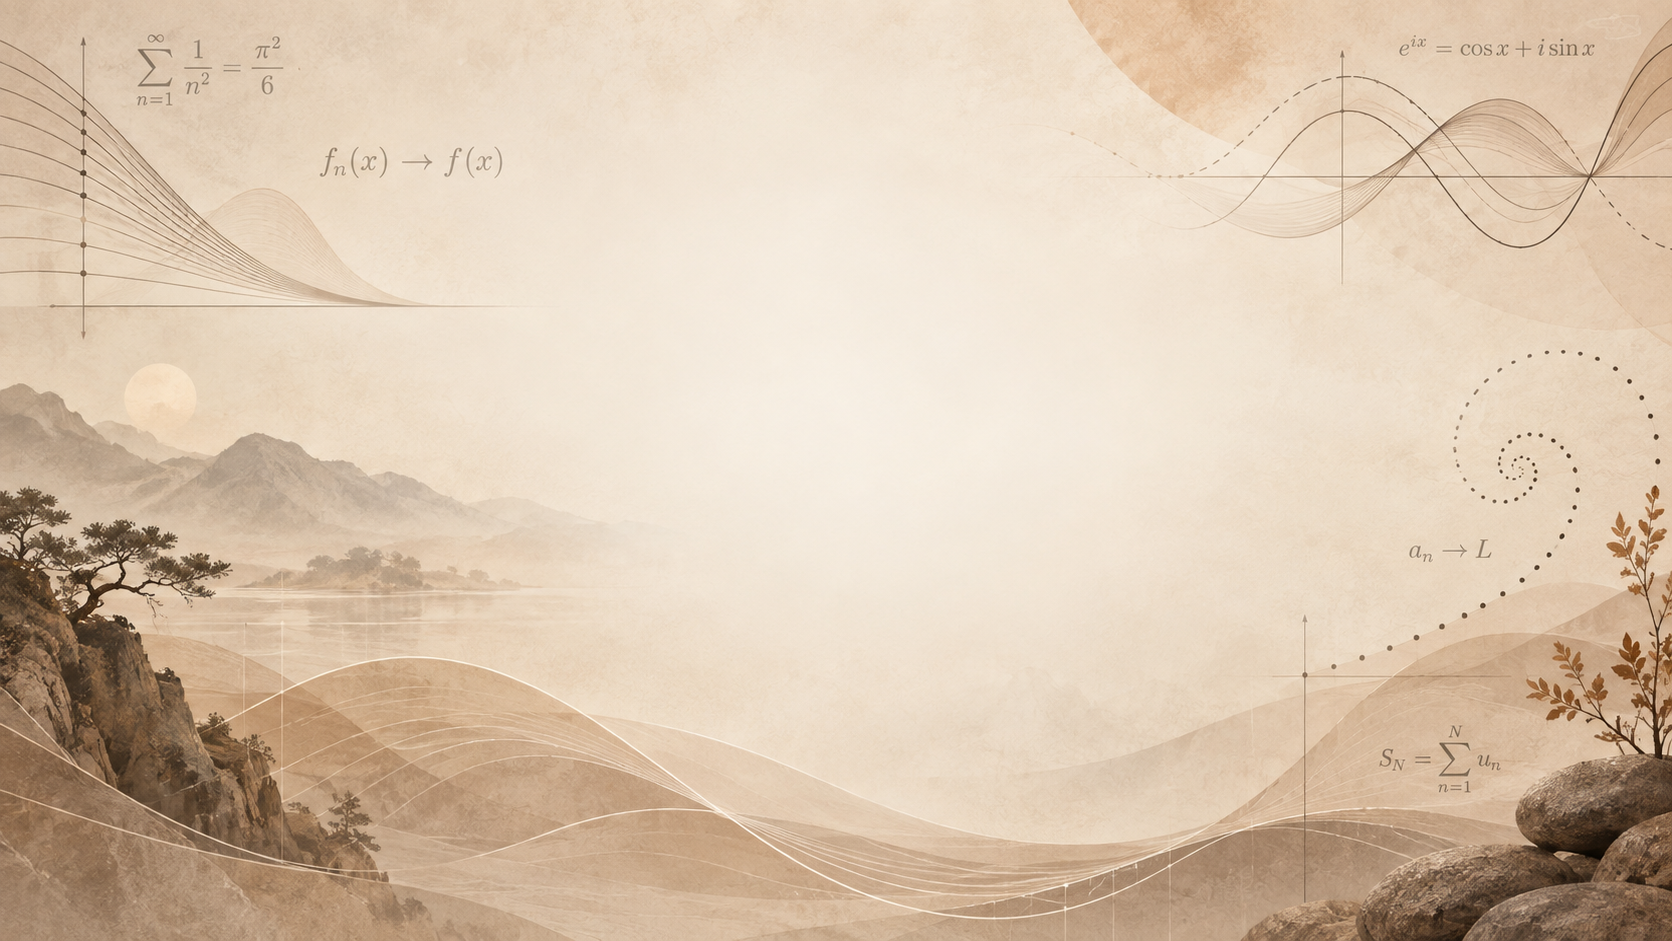
\includegraphics[width=\paperwidth,height=\paperheight,keepaspectratio=false]{chapter_07_bg_00.png}%
}
\begin{frame}[plain]
  \titlepage

  \note{
    Welcome back to Chapter 7, Sequences and Series of Functions. This
    is the fourth section, Uniform Convergence and Integration. In the
    previous section we saw that uniform convergence preserves
    continuity. Now we turn to integrals. We will prove that a uniform
    limit of integrable functions is integrable, and that the integral
    of the limit is the limit of the integrals. As a corollary, a
    uniformly convergent series can be integrated term by term. The
    section is short, but the result is used constantly in the rest of
    the book. Let's begin.
  }
\end{frame}
}

{
\usebackgroundtemplate{%
  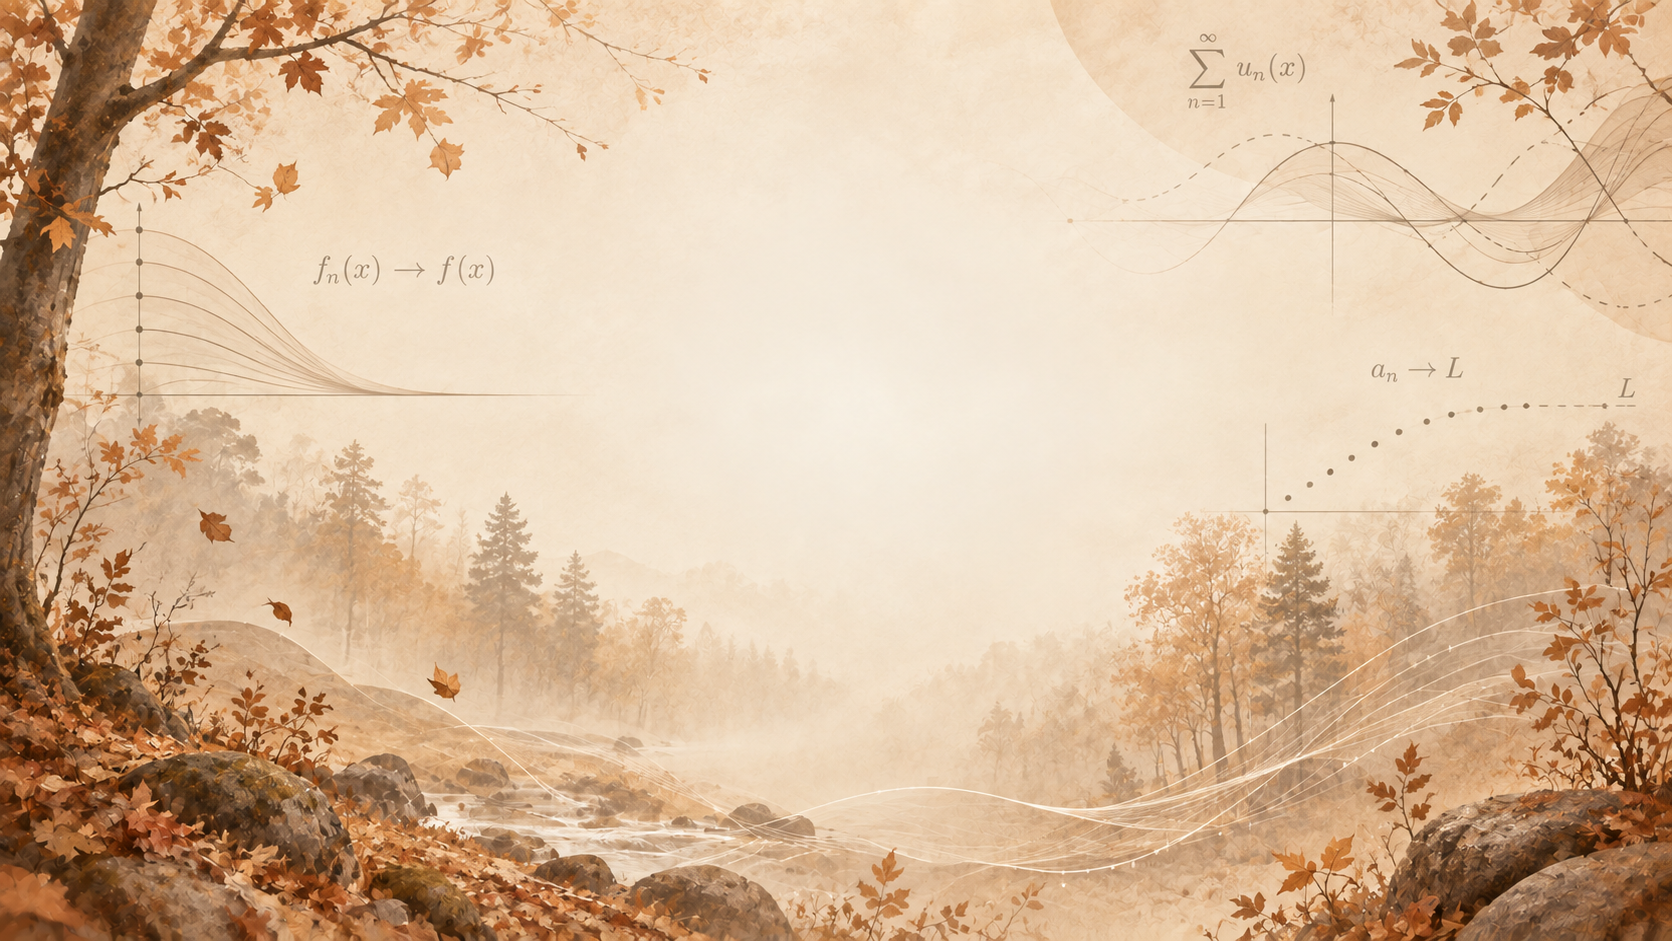
\includegraphics[width=\paperwidth,height=\paperheight,keepaspectratio=false]{chapter_07_bg_01.png}%
}
\begin{frame}[c]{Outline}
  \begin{center}
    \tableofcontents
  \end{center}

  \note{
    Here is the plan. After a short motivation, in which we recall what
    went wrong in Example 7.6, we state Theorem 7.16, the main result of
    this section. Then we prove it in a few steps, using upper and lower
    integrals from Chapter 6. Next comes the corollary on term by term
    integration of series, with an example. We then collect a few
    remarks that explain the role of each hypothesis, and close with a
    summary.
  }
\end{frame}

\section{Motivation}

% --- Build 1/3 ---
\begin{frame}{Why This Section Matters}
  \begin{hlbox}
  \begin{itemize}
    \item The \alert{main problem} of Section 7.1, now for integrals:
      \[
        \lim_{n \to \infty} \int_a^b f_n \, d\alpha
        \;\overset{?}{=}\;
        \int_a^b \Bigl( \lim_{n \to \infty} f_n \Bigr) d\alpha
      \]
  \end{itemize}
  \end{hlbox}

  \note{
    Recall the main problem of this chapter: when do properties of the
    functions "f" sub "n" pass to the limit function? For integration,
    the question is the identity on the slide. On the left, we integrate
    each "f" sub "n" first and then take the limit of the resulting
    numbers. On the right, we first form the limit function and then
    integrate it. In other words, can the limit and the integral be
    interchanged? And before that, is the limit function even
    integrable?
  }
\end{frame}

% --- Build 2/3 ---
\begin{frame}{Why This Section Matters}
  \begin{hlbox}
  \begin{itemize}
    \item The \alert{main problem} of Section 7.1, now for integrals:
      \[
        \lim_{n \to \infty} \int_a^b f_n \, d\alpha
        \;\overset{?}{=}\;
        \int_a^b \Bigl( \lim_{n \to \infty} f_n \Bigr) d\alpha
      \]
    \item Under \emph{pointwise} convergence: \alert{no}.\\
      Example 7.6: integrals tend to $\tfrac12$, the limit function is $0$
  \end{itemize}
  \end{hlbox}

  \note{
    Under pointwise convergence the answer is no. In Example 7.6 we met
    a sequence of functions on the unit interval that converges to zero
    at every single point, yet whose integrals converge to one half
    rather than to zero. So the limit of the integrals and the integral
    of the limit can both be finite and still disagree. We will look at
    this example again in a moment.
  }
\end{frame}

% --- Build 3/3 ---
\begin{frame}{Why This Section Matters}
  \begin{hlbox}
  \begin{itemize}
    \item The \alert{main problem} of Section 7.1, now for integrals:
      \[
        \lim_{n \to \infty} \int_a^b f_n \, d\alpha
        \;\overset{?}{=}\;
        \int_a^b \Bigl( \lim_{n \to \infty} f_n \Bigr) d\alpha
      \]
    \item Under \emph{pointwise} convergence: \alert{no}.\\
      Example 7.6: integrals tend to $\tfrac12$, the limit function is $0$
    \item Under \emph{uniform} convergence on $[a,b]$: \alert{yes!}
  \end{itemize}
  \end{hlbox}

  \note{
    The good news of this section is that uniform convergence on a
    closed bounded interval fixes the problem. Just as it allowed us to
    interchange two limits in the previous section, it allows us to
    interchange a limit and an integral here. And this works for the
    general Riemann Stieltjes integral with respect to any increasing
    function alpha, not only for the ordinary Riemann integral.
  }
\end{frame}

\begin{frame}{Recall Example 7.6: Bumps That Do Not Vanish}
  \begin{columns}[T]
    \begin{column}{0.56\textwidth}
      \begin{tikzpicture}
        \begin{axis}[
          axis background/.style={fill=white, fill opacity=0.6},
          width=8.2cm, height=5.6cm,
          xmin=0, xmax=1.02, ymin=0, ymax=4.2,
          axis lines=left, axis line style={gray!75},
          xtick={0,0.5,1}, ytick={0,1,2,3,4},
          tick label style={font=\scriptsize},
          every axis plot/.append style={curveln},
        ]
          \addplot[name path=g80, domain=0:1, samples=400, thmcolor] {bump(x,80)};
          \addplot[name path=g20, domain=0:1, samples=300, excolor] {bump(x,20)};
          \addplot[name path=g5, domain=0:1, samples=200, defcolor] {bump(x,5)};
          \path[name path=xaxis] (axis cs:0,0) -- (axis cs:1,0);
          \addplot[thmcolor!25, opacity=0.6] fill between[of=g80 and xaxis];
          \node[font=\scriptsize, defcolor] at (axis cs:0.62,1.15) {$n=5$};
          \node[font=\scriptsize, excolor] at (axis cs:0.36,2.15) {$n=20$};
          \node[font=\scriptsize, thmcolor] at (axis cs:0.24,3.75) {$n=80$};
        \end{axis}
      \end{tikzpicture}
    \end{column}
    \begin{column}{0.42\textwidth}
      \begin{exblock}{Example 7.6 (with $n$)}
        $f_n(x) = n\,x(1-x^2)^n$ on $[0,1]$
        \[
          f_n(x) \to 0 \quad (0 \le x \le 1)
        \]
        \[
          \int_0^1 f_n\,dx = \frac{n}{2n+2} \to \frac12
        \]
      \end{exblock}
      \begin{remblock}{Rudin's first version}
        With $n^2$ in place of $n$:
        \[
          \int_0^1 f_n\,dx = \frac{n^2}{2n+2} \to +\infty
        \]
      \end{remblock}
    \end{column}
  \end{columns}

  \note{
    Here is Example 7.6, in the version with "n" instead of "n" squared.
    The plot shows "f" sub "n" for "n" equal to 5 in blue, 20 in brown,
    and 80 in red. Each graph is a bump that moves toward the origin
    and becomes taller and thinner. At every fixed point the values tend
    to zero, so the limit function is identically zero. But the area
    under each bump, shaded for the red curve, stays close to one half.
    The mass does not disappear; it concentrates near zero. The tall
    peaks are exactly what prevents the convergence from being uniform.
    The gray box adds that Rudin first used "n" squared in place of "n";
    then the integrals even tend to infinity.
  }
\end{frame}

\begin{frame}{Roadmap of This Section}
  \vspace{0.6em}
  \begin{center}
  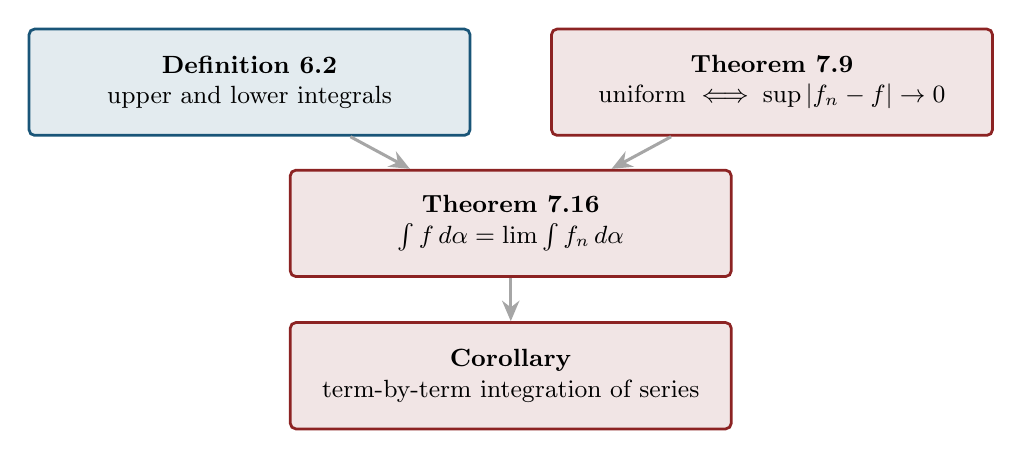
\begin{tikzpicture}[node distance=0.55cm and 1.0cm]
    \node[box=defcolor] (a) {\textbf{Definition 6.2}\\ upper and lower integrals};
    \node[box=thmcolor, right=of a] (b) {\textbf{Theorem 7.9}\\ uniform $\iff \sup |f_n - f| \to 0$};
    \node[box=thmcolor, below=1.1cm of $(a)!0.5!(b)$] (c) {\textbf{Theorem 7.16}\\ $\int f\,d\alpha = \lim \int f_n\,d\alpha$};
    \node[box=thmcolor, below=of c] (d) {\textbf{Corollary}\\ term-by-term integration of series};
    \draw[guide, gray!70] (a) -- (c);
    \draw[guide, gray!70] (b) -- (c);
    \draw[guide, gray!70] (c) -- (d);
  \end{tikzpicture}
  \end{center}

  \note{
    The diagram shows the structure of this section. In the top row are
    two tools we already have. On the left, in blue, Definition 6.2 from
    Chapter 6: upper and lower integrals. On the right, in red, Theorem
    7.9: uniform convergence means that the supremum of the distance
    between "f" sub "n" and "f" tends to zero. Gray arrows lead from both
    to the main result, Theorem 7.16, which says that the integral of
    the limit equals the limit of the integrals. Another arrow leads
    down to its corollary about integrating series term by term. Let's
    state the theorem.
  }
\end{frame}
}

{
\usebackgroundtemplate{%
  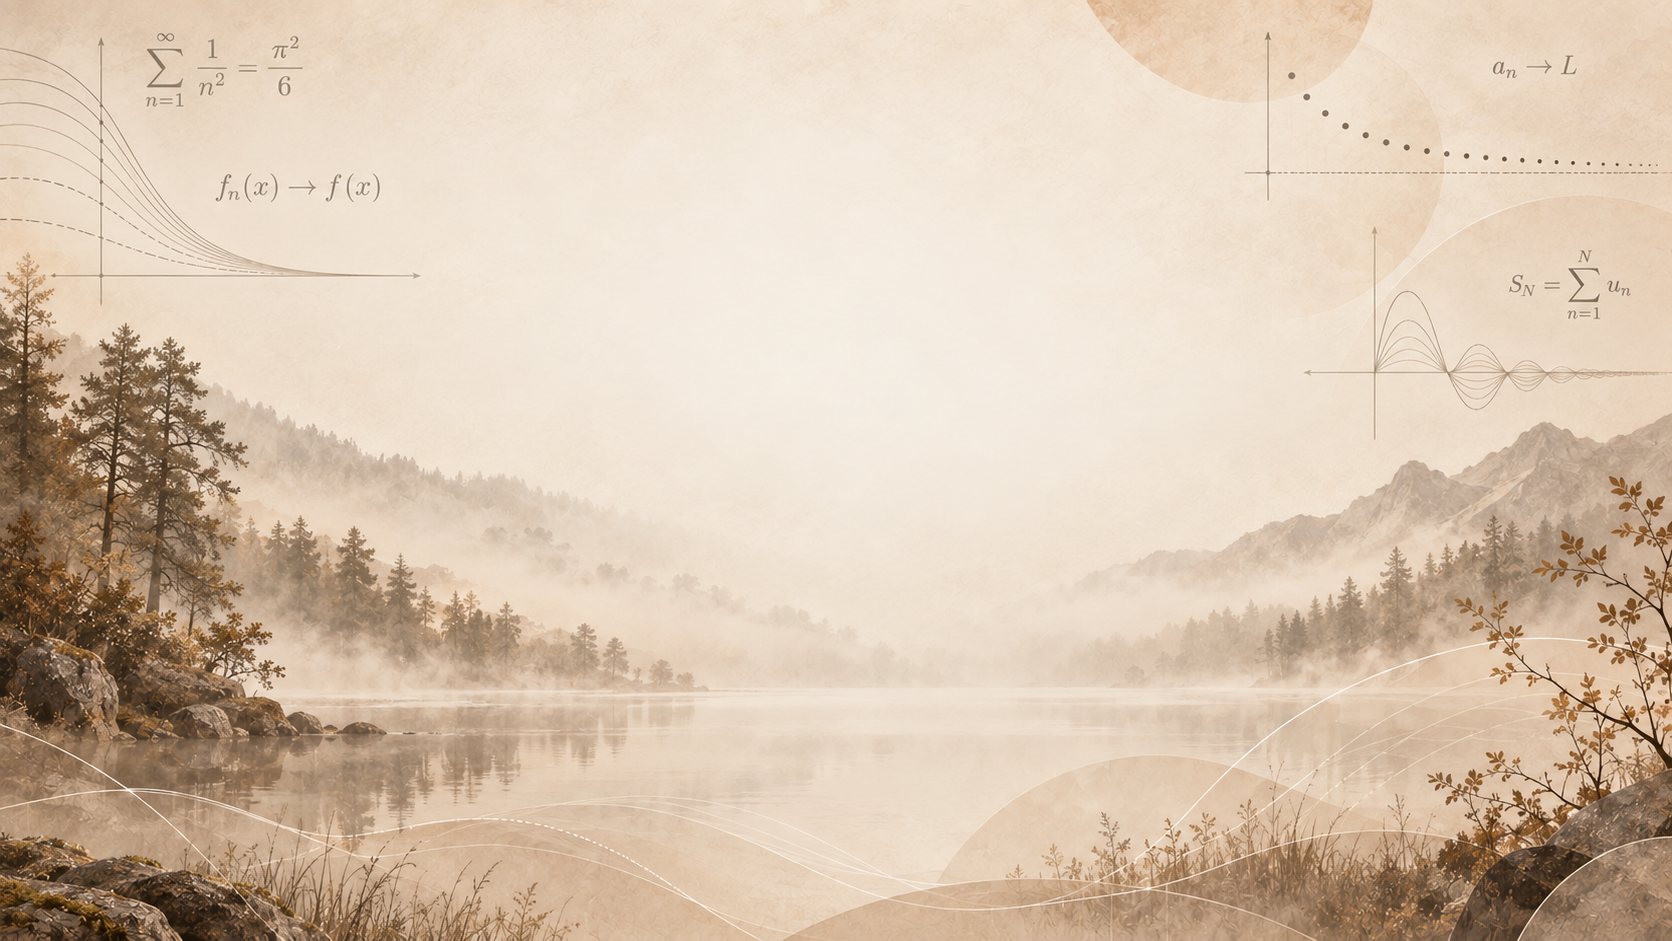
\includegraphics[width=\paperwidth,height=\paperheight,keepaspectratio=false]{chapter_07_bg_02.png}%
}
\section{Theorem 7.16}

% --- Build 1/2 ---
\begin{frame}{Theorem 7.16: Limit of Integrals}
  \begin{thmblock}{Theorem 7.16}
    Let $\alpha$ be monotonically increasing on $[a, b]$. Suppose
    $f_n \in \mathscr{R}(\alpha)$ on $[a, b]$, for $n = 1, 2, 3, \dots$,
    and suppose $f_n \to f$ \alert{uniformly} on $[a, b]$. Then
    $f \in \mathscr{R}(\alpha)$ on $[a, b]$, and
    \begin{equation}
      \int_a^b f\,d\alpha = \lim_{n \to \infty} \int_a^b f_n\,d\alpha. \tag{23}
    \end{equation}
  \end{thmblock}

  \note{
    Here is Theorem 7.16. We fix an increasing function alpha on the
    closed interval from "a" to "b". Each "f" sub "n" is Riemann
    Stieltjes integrable with respect to alpha, which is what script
    capital "R" of alpha means, and the sequence converges uniformly to
    a function "f". The conclusion has two parts. First, "f" is again
    integrable with respect to alpha. Second, equation 23: the integral
    of "f" equals the limit of the integrals of "f" sub "n".
  }
\end{frame}

% --- Build 2/2 ---
\begin{frame}{Theorem 7.16: Limit of Integrals}
  \begin{thmblock}{Theorem 7.16}
    Let $\alpha$ be monotonically increasing on $[a, b]$. Suppose
    $f_n \in \mathscr{R}(\alpha)$ on $[a, b]$, for $n = 1, 2, 3, \dots$,
    and suppose $f_n \to f$ \alert{uniformly} on $[a, b]$. Then
    $f \in \mathscr{R}(\alpha)$ on $[a, b]$, and
    \begin{equation}
      \int_a^b f\,d\alpha = \lim_{n \to \infty} \int_a^b f_n\,d\alpha. \tag{23}
    \end{equation}
  \end{thmblock}
  \begin{remblock}{Three conclusions in one}
    \textbf{(i)} $f$ is integrable \quad
    \textbf{(ii)} the limit on the right \alert{exists} \quad
    \textbf{(iii)} they are equal
  \end{remblock}

  \note{
    It is worth unpacking how much the theorem says. As Rudin points
    out, the existence of the limit on the right is part of the
    conclusion, not an assumption. So there are really three claims, as
    the gray box lists. Claim 1: "f" is integrable, which is not obvious
    at all, since "f" is only defined as a limit. Claim 2: the integrals
    of "f" sub "n" form a convergent sequence of numbers. Claim 3: that
    limit is exactly the integral of "f". Let's look more closely at
    the first claim.
  }
\end{frame}

\begin{frame}{Why Integrability of $f$ Is Not Free}
  \begin{remblock}{Remark}
    \begin{itemize}
      \item If the $f_n$ are \emph{continuous}: $f$ is continuous (Theorem 7.12),
        hence $f \in \mathscr{R}(\alpha)$ (Theorem 6.8). Easy.
      \item But $f_n \in \mathscr{R}(\alpha)$ may be \alert{discontinuous}.
        Example 7.4: each $f_m$ is nonzero at finitely many points of $[0,1]$,
        so $f_m \in \mathscr{R}$, yet
        \[
          \lim_{m \to \infty} f_m(x) =
          \begin{cases} 1 & x \text{ rational} \\ 0 & x \text{ irrational} \end{cases}
          \quad \text{is \alert{not} Riemann-integrable.}
        \]
    \end{itemize}
  \end{remblock}

  \note{
    Why is the first claim, integrability of "f", worth stating? If
    every "f" sub "n" is continuous, it comes for free: the uniform limit
    is continuous by Theorem 7.12, and continuous functions are
    integrable by Theorem 6.8. But integrable functions may be
    discontinuous, and then a pointwise limit can be badly behaved.
    Recall Example 7.4: each "f" sub "m" equals 1 at finitely many points
    of the unit interval and zero elsewhere, so it is integrable. Yet the
    pointwise limit is 1 at rationals and zero at irrationals, which is
    not Riemann integrable. So integrability of "f" genuinely depends on
    uniform convergence. Now let's see why uniformity is enough.
  }
\end{frame}

\begin{frame}{The Picture: $f$ Trapped in a Thin Tube}
  \begin{center}
  \begin{tikzpicture}
    \begin{axis}[
          axis background/.style={fill=white, fill opacity=0.6},
      width=12.5cm, height=5.4cm,
      xmin=0, xmax=7.2, ymin=0, ymax=4.6,
      axis lines=left, axis line style={gray!75},
      xtick={0.5,6.8}, xticklabels={$a$,$b$}, ytick=\empty,
      tick label style={font=\footnotesize}, clip=false,
    ]
      \addplot[name path=up, domain=0.5:6.8, samples=120, draw=none] {tubefn(x)+0.45};
      \addplot[name path=lo, domain=0.5:6.8, samples=120, draw=none] {tubefn(x)-0.45};
      \addplot[defcolor!25, opacity=0.8] fill between[of=up and lo];
      \addplot[domain=0.5:6.8, samples=120, defcolor, projln] {tubefn(x)+0.45};
      \addplot[domain=0.5:6.8, samples=120, defcolor, projln] {tubefn(x)-0.45};
      \addplot[domain=0.5:6.8, samples=120, defcolor, curveln] {tubefn(x)};
      \addplot[domain=0.5:6.8, samples=300, thmcolor, curveln, line width=1.2pt] {tubef(x)};
      \node[font=\footnotesize, text=defcolor, anchor=west, fill=white, fill opacity=0.65, text opacity=1, inner sep=1pt] at (axis cs:6.85,3.38) {$f_n + \varepsilon_n$};
      \node[font=\footnotesize, text=defcolor, anchor=west, fill=white, fill opacity=0.65, text opacity=1, inner sep=1pt] at (axis cs:6.85,2.88) {$f_n$};
      \node[font=\footnotesize, text=defcolor, anchor=west, fill=white, fill opacity=0.65, text opacity=1, inner sep=1pt] at (axis cs:6.85,2.38) {$f_n - \varepsilon_n$};
      \node[font=\footnotesize, thmcolor] at (axis cs:2.2,3.75) {$f$};
      \draw[<->, gray, line width=0.8pt] (axis cs:4.6,{tubefn(4.6)-0.45}) -- (axis cs:4.6,{tubefn(4.6)+0.45});
      \node[font=\scriptsize, below=1pt] at (axis cs:4.6,{tubefn(4.6)-0.45}) {$2\varepsilon_n$};
    \end{axis}
  \end{tikzpicture}
  \end{center}

  \note{
    Here is the key picture. The solid blue curve is "f" sub "n" for
    some fixed large "n". The shaded blue tube around it, bounded by the
    dashed curves, consists of all values within epsilon sub "n" of "f"
    sub "n"; its total height is 2 epsilon sub "n", as the gray arrow
    shows. Uniform convergence means that for large "n" the limit
    function "f", the red wiggly curve, lies entirely inside this tube.
    The area under "f", whatever it is, is therefore squeezed between
    the areas under the two dashed curves, and those differ by very
    little. As "n" grows, the tube shrinks to zero thickness. That is
    the whole idea of the proof.
  }
\end{frame}
}

{
\usebackgroundtemplate{%
  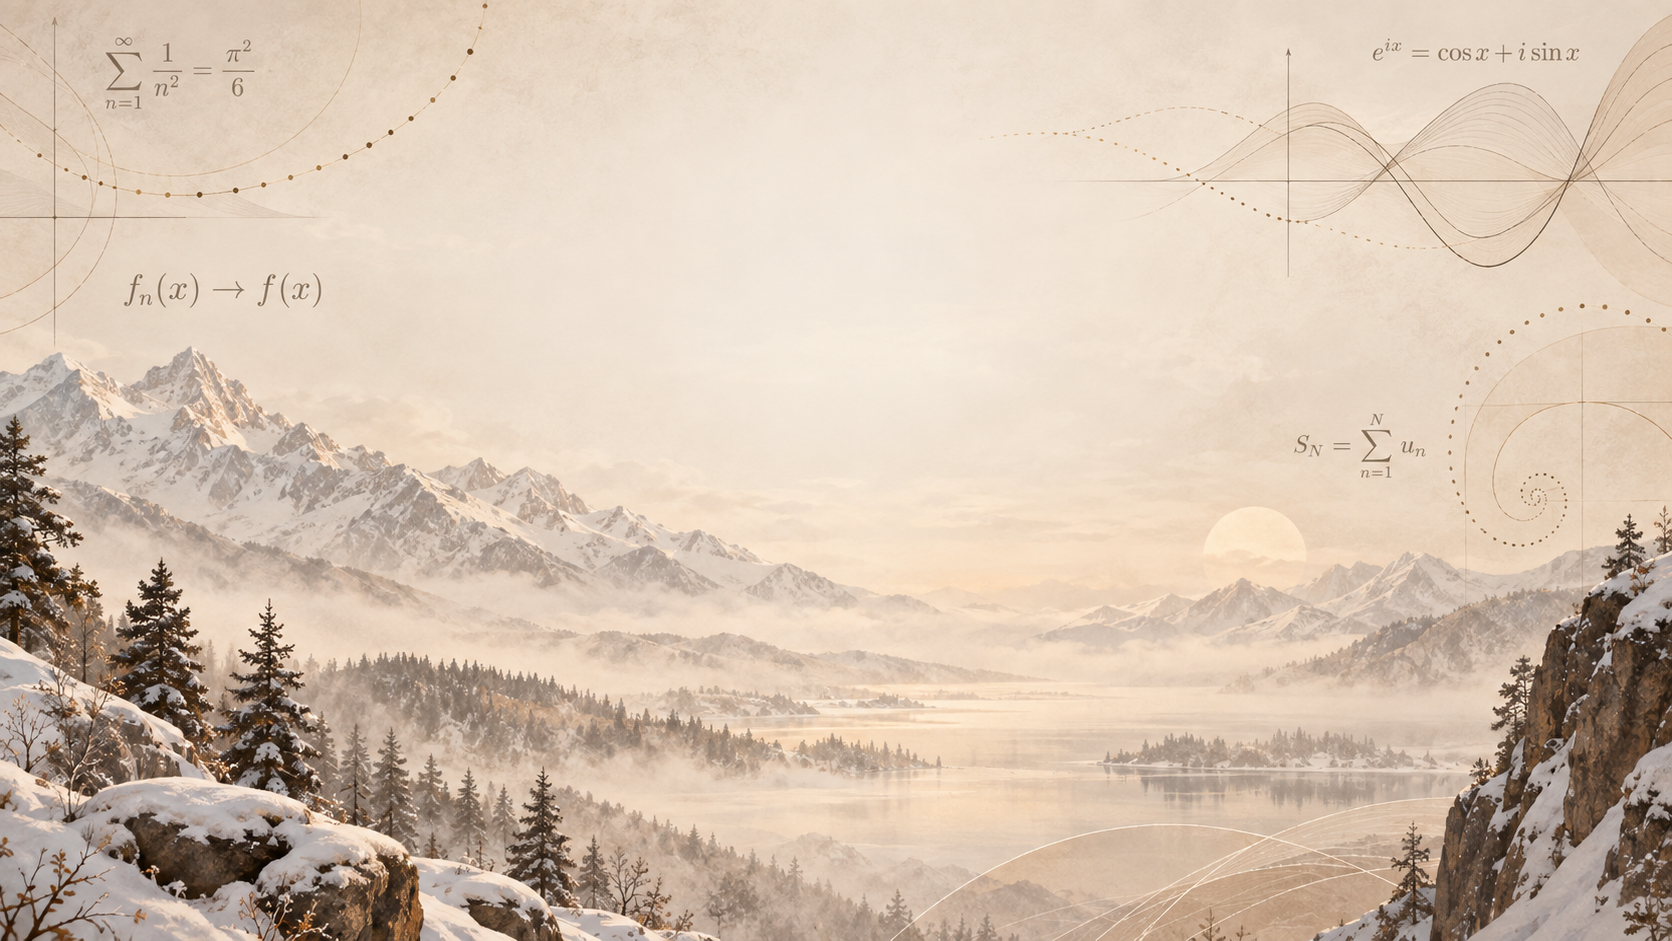
\includegraphics[width=\paperwidth,height=\paperheight,keepaspectratio=false]{chapter_07_bg_03.png}%
}
\section{Proof of Theorem 7.16}

% --- Build 1/3 ---
\begin{frame}{Proof Strategy: Theorem 7.16}
  \begin{hlbox}
  \textbf{Goal:} $f \in \mathscr{R}(\alpha)$ and
  $\int_a^b f_n\,d\alpha \to \int_a^b f\,d\alpha$.

  \vspace{0.6em}
  \textbf{Approach:}
  \begin{enumerate}
    \item Trap $f$ in a \alert{tube}: $f_n - \varepsilon_n \le f \le f_n + \varepsilon_n$.
  \end{enumerate}
  \end{hlbox}

  \note{
    Let's lay out the strategy before the formal proof. The goal is the
    pair of conclusions: "f" is integrable, and the integrals converge to
    the integral of "f". The first step makes the picture precise: we
    measure how far "f" sub "n" is from "f" by a single number, epsilon
    sub "n", and then "f" is trapped between "f" sub "n" minus epsilon
    sub "n" and "f" sub "n" plus epsilon sub "n".
  }
\end{frame}

% --- Build 2/3 ---
\begin{frame}{Proof Strategy: Theorem 7.16}
  \begin{hlbox}
  \textbf{Goal:} $f \in \mathscr{R}(\alpha)$ and
  $\int_a^b f_n\,d\alpha \to \int_a^b f\,d\alpha$.

  \vspace{0.6em}
  \textbf{Approach:}
  \begin{enumerate}
    \item Trap $f$ in a \alert{tube}: $f_n - \varepsilon_n \le f \le f_n + \varepsilon_n$.
    \item Sandwich the \alert{upper and lower integrals} of $f$; \\
    their gap $\to 0$, so $f \in \mathscr{R}(\alpha)$.
  \end{enumerate}
  \end{hlbox}

  \note{
    Second, we cannot integrate "f" yet, because we do not know that it
    is integrable. But upper and lower integrals exist for any bounded
    function. Integrating the tube inequality, we squeeze both the upper
    and the lower integral of "f" between two numbers that are very
    close together. Letting "n" go to infinity forces the upper and
    lower integrals to coincide, which is exactly integrability.
  }
\end{frame}

% --- Build 3/3 ---
\begin{frame}{Proof Strategy: Theorem 7.16}
  \begin{hlbox}
  \textbf{Goal:} $f \in \mathscr{R}(\alpha)$ and
  $\int_a^b f_n\,d\alpha \to \int_a^b f\,d\alpha$.

  \vspace{0.6em}
  \textbf{Approach:}
  \begin{enumerate}
    \item Trap $f$ in a \alert{tube}: $f_n - \varepsilon_n \le f \le f_n + \varepsilon_n$.
    \item Sandwich the \alert{upper and lower integrals} of $f$; \\
    their gap $\to 0$, so $f \in \mathscr{R}(\alpha)$.
    \item The same sandwich gives \\
      $\bigl|\int f\,d\alpha - \int f_n\,d\alpha\bigr| \le \varepsilon_n [\alpha(b) - \alpha(a)] \to 0$.
  \end{enumerate}
  \end{hlbox}

  \note{
    Third, once "f" is known to be integrable, the very same sandwich
    tells us that the integral of "f" and the integral of "f" sub "n"
    are within epsilon sub "n" times alpha of "b" minus alpha of "a" of
    each other. Since epsilon sub "n" tends to zero, the integrals
    converge. Before carrying this out, let's recall the two tools we
    need.
  }
\end{frame}

% --- Build 1/2 ---
\begin{frame}{Tools We Need}
  \begin{defblock}{Recall: Definition 6.2 (upper and lower integrals)}
    For bounded $f$ on $[a,b]$:
    \[
      \overline{\int_a^b} f\,d\alpha = \inf_P U(P, f, \alpha), \qquad
      \underline{\int_a^b} f\,d\alpha = \sup_P L(P, f, \alpha).
    \]
    $f \in \mathscr{R}(\alpha)$ $\iff$ the two are \alert{equal}. \\
    \textbf{Consequence:} $g \le h \Rightarrow$ upper/lower integrals of $g$ $\le$ those of $h$.
  \end{defblock}

  \note{
    First, Definition 6.2. For any bounded function, the upper integral
    is the infimum of the upper sums over all partitions, and the lower
    integral is the supremum of the lower sums. These always exist, and
    the function is integrable precisely when the two coincide. We also
    use a simple consequence of the definition, monotonicity: if "g" is
    at most "h" everywhere,
    then every upper or lower sum of "g" is at most the corresponding
    sum of "h", so the upper and lower integrals of "g" are at most
    those of "h".
  }
\end{frame}

% --- Build 2/2 ---
\begin{frame}{Tools We Need}
  \begin{defblock}{Recall: Definition 6.2 (upper and lower integrals)}
    For bounded $f$ on $[a,b]$:
    \[
      \overline{\int_a^b} f\,d\alpha = \inf_P U(P, f, \alpha), \qquad
      \underline{\int_a^b} f\,d\alpha = \sup_P L(P, f, \alpha).
    \]
    $f \in \mathscr{R}(\alpha)$ $\iff$ the two are \alert{equal}. \\
    \textbf{Consequence:} $g \le h \Rightarrow$ upper/lower integrals of $g$ $\le$ those of $h$.
  \end{defblock}
  \begin{thmblock}{Recall: Theorem 7.9}
    $f_n \to f$ uniformly on $E$ $\iff$
    $\displaystyle M_n = \sup_{x \in E} |f_n(x) - f(x)| \to 0$.
  \end{thmblock}

  \note{
    Second, Theorem 7.9 from Section 7.2. Uniform convergence on a set
    capital "E" is equivalent to the statement that the numbers capital
    "M" sub "n", the supremum over capital "E" of the distance between
    "f" sub "n" and "f", tend to zero. In other words, the worst case
    error goes to zero. With these two tools in hand, let's start the
    proof.
  }
\end{frame}

% --- Build 1/2 ---
\begin{frame}{Proof of Theorem 7.16}
  \begin{proofblock}{Step 1: Reduce to real $f_n$; measure the error}
    Real and imaginary parts are treated separately, so assume $f_n$ \alert{real}. Put
    \begin{equation}
      \varepsilon_n = \sup_{a \le x \le b} |f_n(x) - f(x)|. \tag{24}
    \end{equation}
    By Theorem 7.9, $\varepsilon_n \to 0$ as $n \to \infty$.
  \end{proofblock}

  \note{
    Step 1. It suffices to prove the theorem for real functions: a
    complex function is integrable when its real and imaginary parts
    are, its integral is computed part by part, and uniform convergence
    of "f" sub "n" gives uniform convergence of both parts. So we assume
    everything is real. Then we define epsilon sub "n" as in equation
    24: the largest deviation of "f" sub "n" from "f" over the interval.
    By Theorem 7.9, uniform convergence means precisely that epsilon sub
    "n" tends to zero. In particular, epsilon sub "n" is finite for all
    large "n", and those are the only "n" we care about.
  }
\end{frame}

% --- Build 2/2 ---
\begin{frame}{Proof of Theorem 7.16}
  \begin{proofblock}{Step 1: Reduce to real $f_n$; measure the error}
    Real and imaginary parts are treated separately, so assume $f_n$ \alert{real}. Put
    \begin{equation}
      \varepsilon_n = \sup_{a \le x \le b} |f_n(x) - f(x)|. \tag{24}
    \end{equation}
    By Theorem 7.9, $\varepsilon_n \to 0$ as $n \to \infty$.
  \end{proofblock}
  \begin{proofblock}{Step 2: The tube}
    For every $x \in [a,b]$:
    \qquad $\boxed{f_n(x) - \varepsilon_n \le f(x) \le f_n(x) + \varepsilon_n.}$
  \end{proofblock}

  \note{
    Step 2 is the tube from our picture. Since epsilon sub "n" bounds the
    distance between "f" sub "n" of "x" and "f" of "x" at every point,
    the value of "f" at "x" lies between "f" sub "n" of "x" minus epsilon
    sub "n" and "f" sub "n" of "x" plus epsilon sub "n". Notice one useful
    consequence: since "f" sub "n" is integrable, it is bounded, and
    therefore "f" is bounded too. So the upper and lower integrals of
    "f" make sense.
  }
\end{frame}

% --- Build 1/2 ---
\begin{frame}{Proof of Theorem 7.16}
  \begin{proofblock}{Step 3: Integrate the tube (monotonicity)}
    \begin{equation}
      \int_a^b (f_n - \varepsilon_n)\,d\alpha
      \le \underline{\int_a^b} f\,d\alpha
      \le \overline{\int_a^b} f\,d\alpha
      \le \int_a^b (f_n + \varepsilon_n)\,d\alpha. \tag{25}
    \end{equation}
    Outer inequalities: \alert{monotonicity}. \ Middle inequality: Theorem 6.5.
  \end{proofblock}

  \note{
    Step 3. The two outer functions, "f" sub "n" minus epsilon sub "n"
    and "f" sub "n" plus epsilon sub "n", are integrable, being an
    integrable function plus a constant. As the last line of the box
    says, the outer inequalities come from monotonicity: the lower
    integral of "f" is at least the integral of the lower edge of the
    tube, and the upper integral of "f" is at most the integral of the
    upper edge. The middle one is Theorem 6.5: the lower integral never
    exceeds the upper integral. This chain of inequalities is equation
    25, the heart of the proof.
  }
\end{frame}

% --- Build 2/2 ---
\begin{frame}{Proof of Theorem 7.16}
  \begin{proofblock}{Step 3: Integrate the tube (monotonicity)}
    \begin{equation}
      \int_a^b (f_n - \varepsilon_n)\,d\alpha
      \le \underline{\int_a^b} f\,d\alpha
      \le \overline{\int_a^b} f\,d\alpha
      \le \int_a^b (f_n + \varepsilon_n)\,d\alpha. \tag{25}
    \end{equation}
    Outer inequalities: \alert{monotonicity}. \ Middle inequality: Theorem 6.5.
  \end{proofblock}

  \vspace{0.2em}
  \begin{center}
  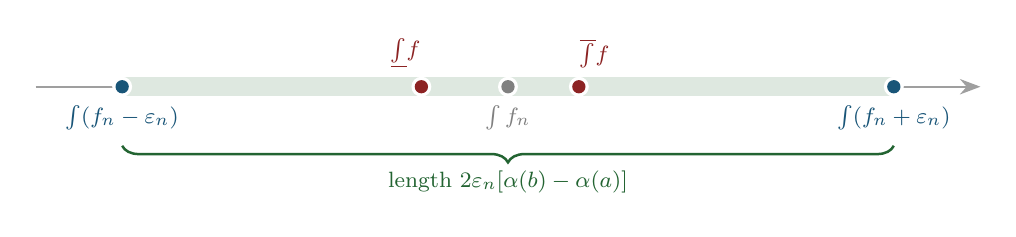
\begin{tikzpicture}[x=1cm,y=1cm, every node/.append style={fill=white, fill opacity=0.65, text opacity=1, inner sep=1.5pt}]
    \fill[white, opacity=0.5] (-0.7,-1.55) rectangle (11.5,0.75);
    \draw[axisln] (-0.6,0) -- (11.4,0);
    \fill[proofcolor!15] (0.5,-0.12) rectangle (10.3,0.12);
    \dotpt{defcolor}{(0.5,0)}
    \dotpt{thmcolor}{(4.3,0)}
    \dotpt{thmcolor}{(6.3,0)}
    \dotpt{defcolor}{(10.3,0)}
    \dotpt{gray}{(5.4,0)}
    \node[below=5pt, font=\footnotesize, text=defcolor] at (0.5,0) {$\int (f_n - \varepsilon_n)$};
    \node[above=5pt, font=\footnotesize, text=thmcolor] at (4.1,0) {$\underline{\int} f$};
    \node[above=5pt, font=\footnotesize, text=thmcolor] at (6.5,0) {$\overline{\int} f$};
    \node[below=5pt, font=\footnotesize, text=defcolor] at (10.3,0) {$\int (f_n + \varepsilon_n)$};
    \node[below=5pt, font=\footnotesize, text=gray] at (5.4,0) {$\int f_n$};
    \draw[decorate, decoration={brace, amplitude=6pt, mirror}, proofcolor, line width=0.9pt]
      (0.5,-0.75) -- node[below=7pt, font=\footnotesize, text=proofcolor] {length $2\varepsilon_n[\alpha(b) - \alpha(a)]$} (10.3,-0.75);
  \end{tikzpicture}
  \end{center}

  \note{
    The number line shows equation 25. The two blue points are the
    integrals of the lower and upper edges of the tube, and the gray
    point between them is the integral of "f" sub "n". Integrating the
    constant epsilon sub "n" gives epsilon sub "n" times alpha of "b"
    minus alpha of "a", so the blue points sit exactly that far to the
    left and right of the gray one.
    The green brace marks the whole interval, of length 2 epsilon sub
    "n" times alpha of "b" minus alpha of "a". The two red points, the
    lower and upper integrals of "f", are trapped inside it.
  }
\end{frame}

\begin{frame}{Proof of Theorem 7.16}
  \begin{proofblock}{Step 4: The gap closes, so $f \in \mathscr{R}(\alpha)$}
    Subtracting the outer ends of (25):
    \[
      0 \le \overline{\int_a^b} f\,d\alpha - \underline{\int_a^b} f\,d\alpha
      \le 2\varepsilon_n[\alpha(b) - \alpha(a)]
      \xrightarrow[n \to \infty]{} 0.
    \]
    The left side does not depend on $n$, so it is $0$:
    \quad $\boxed{f \in \mathscr{R}(\alpha).}$
  \end{proofblock}

  \note{
    Step 4. Both red points lie in the green interval, so their distance
    is at most its length. That is the inequality on the slide: the
    upper integral of "f" minus the lower integral of "f" lies between
    zero and 2 epsilon sub "n" times alpha of "b" minus alpha of "a".
    Here is the crucial observation: the middle quantity does not depend
    on "n" at all, while the right side tends to zero. A fixed
    nonnegative number that is smaller than every term of a sequence
    tending to zero must be zero. So the upper and lower integrals of
    "f" agree, and "f" is integrable. That is the first conclusion.
  }
\end{frame}

% --- Build 1/2 ---
\begin{frame}{Proof of Theorem 7.16}
  \begin{proofblock}{Step 5: The integrals converge}
    Now $\underline{\int} f = \overline{\int} f = \int_a^b f\,d\alpha$, and both
    $\int f\,d\alpha$ and $\int f_n\,d\alpha$ lie in the interval of (25):
    \begin{equation}
      \left|\int_a^b f\,d\alpha - \int_a^b f_n\,d\alpha\right|
      \le \varepsilon_n[\alpha(b) - \alpha(a)]. \tag{26}
    \end{equation}
  \end{proofblock}

  \note{
    Step 5. Now that "f" is integrable, its integral is the common value
    of the upper and lower integrals, so it lies in the green interval
    from equation 25. The integral of "f" sub "n" is the midpoint of that
    interval. Two points in an interval, one of them at the center, are
    at most half the length apart. Half the length is epsilon sub "n"
    times alpha of "b" minus alpha of "a". This is equation 26, another
    application of equation 25.
  }
\end{frame}

% --- Build 2/2 ---
\begin{frame}{Proof of Theorem 7.16}
  \begin{proofblock}{Step 5: The integrals converge}
    Now $\underline{\int} f = \overline{\int} f = \int_a^b f\,d\alpha$, and both
    $\int f\,d\alpha$ and $\int f_n\,d\alpha$ lie in the interval of (25):
    \begin{equation}
      \left|\int_a^b f\,d\alpha - \int_a^b f_n\,d\alpha\right|
      \le \varepsilon_n[\alpha(b) - \alpha(a)]. \tag{26}
    \end{equation}
    Since $\varepsilon_n \to 0$, this implies (23):
    \quad $\boxed{\displaystyle \int_a^b f\,d\alpha = \lim_{n \to \infty} \int_a^b f_n\,d\alpha.}$
    \hfill $\blacksquare$
  \end{proofblock}

  \note{
    Finally, as "n" goes to infinity, epsilon sub "n" tends to zero, and
    the factor alpha of "b" minus alpha of "a" is a fixed finite number.
    So the right side of equation 26 tends to zero, which says that the
    integrals of "f" sub "n" converge, and their limit is the integral of
    "f". This is equation 23, and the proof is complete. Notice that the
    estimate 26 is even quantitative: it tells us how fast the integrals
    converge, in terms of the uniform error. Next, let's apply the
    theorem to series.
  }
\end{frame}
}

{
\usebackgroundtemplate{%
  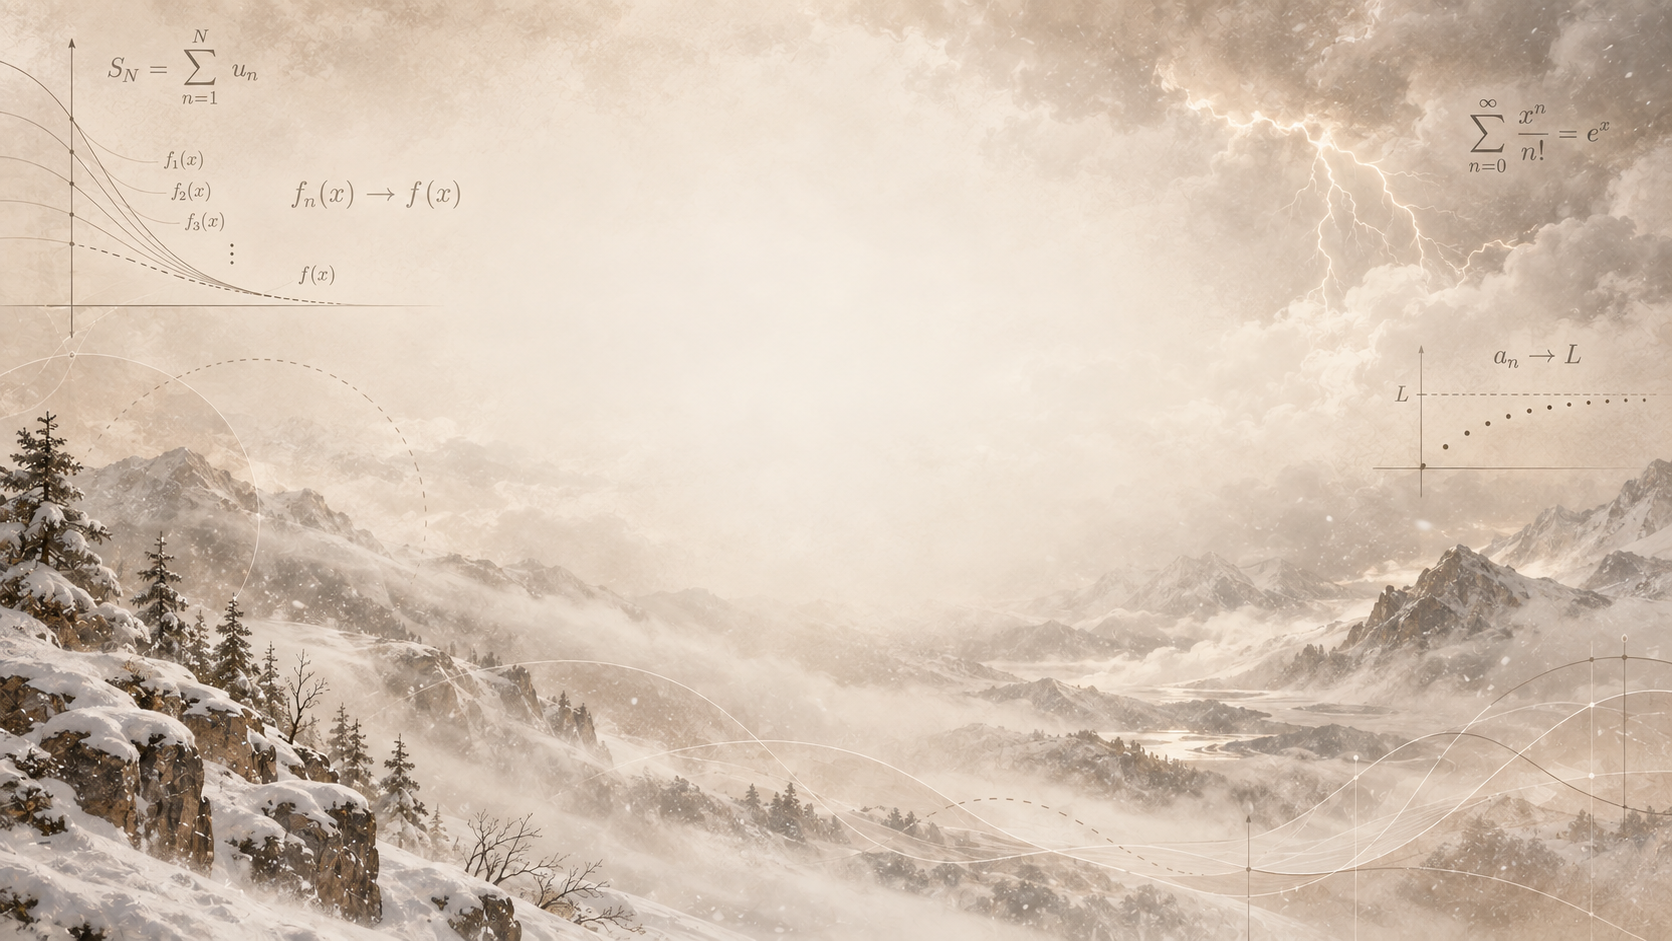
\includegraphics[width=\paperwidth,height=\paperheight,keepaspectratio=false]{chapter_07_bg_04.png}%
}
\section{Term-by-Term Integration}

% --- Build 1/2 ---
\begin{frame}{Corollary: Integrating Series Term by Term}
  \begin{thmblock}{Corollary (Theorem 7.16)}
    If $f_n \in \mathscr{R}(\alpha)$ on $[a, b]$ and if
    $\displaystyle f(x) = \sum_{n=1}^{\infty} f_n(x)$ \ $(a \le x \le b)$,
    the series converging \alert{uniformly} on $[a, b]$, then
    \[
      \int_a^b f\,d\alpha = \sum_{n=1}^{\infty} \int_a^b f_n\,d\alpha.
    \]
  \end{thmblock}

  \note{
    Here is the corollary. Suppose each "f" sub "n" is integrable with
    respect to alpha, and the series of the "f" sub "n" converges
    uniformly on the interval to a function "f". Then the integral of
    the sum equals the sum of the integrals. In other words, as Rudin
    puts it, the series may be integrated term by term. This is one of
    the most frequently used consequences of uniform convergence.
  }
\end{frame}

% --- Build 2/2 ---
\begin{frame}{Corollary: Integrating Series Term by Term}
  \begin{thmblock}{Corollary (Theorem 7.16)}
    If $f_n \in \mathscr{R}(\alpha)$ on $[a, b]$ and if
    $\displaystyle f(x) = \sum_{n=1}^{\infty} f_n(x)$ \ $(a \le x \le b)$,
    the series converging \alert{uniformly} on $[a, b]$, then
    \[
      \int_a^b f\,d\alpha = \sum_{n=1}^{\infty} \int_a^b f_n\,d\alpha.
    \]
  \end{thmblock}
  \begin{proofblock}{Why}
    Partial sums $s_N = \sum_{n=1}^{N} f_n \in \mathscr{R}(\alpha)$ (Theorem 6.12), \\
    $\int s_N\,d\alpha = \sum_{n=1}^{N} \int f_n\,d\alpha$,
    \ $s_N \to f$ uniformly. Apply Theorem 7.16 to $\{s_N\}$.
  \end{proofblock}

  \note{
    The reason is simple. Look at the partial sums "s" sub capital "N",
    the sum of the first capital "N" terms. A finite sum of integrable
    functions is integrable, and its integral is the finite sum of the
    integrals, by the linearity of Theorem 6.12. Uniform convergence of the
    series means, by definition, that the partial sums converge
    uniformly to "f". So Theorem 7.16 applies to the sequence of partial
    sums, and the limit of the finite sums of integrals is the integral
    of "f". That limit is exactly the infinite series of integrals.
  }
\end{frame}

% --- Build 1/2 ---
\begin{frame}{Example: Integrating a Geometric Series}
  \begin{exblock}{Example}
    Fix $0 < x < 1$. On $[0, x]$: \ $|t^n| \le x^n$ and $\sum x^n < \infty$, so
    \[
      \frac{1}{1-t} = \sum_{n=0}^{\infty} t^n
      \quad \text{\alert{uniformly} on } [0, x] \quad \text{(Theorem 7.10)}.
    \]
  \end{exblock}

  \note{
    Let's see the corollary in action. Fix a number "x" strictly between
    zero and 1, and consider the geometric series, the sum of "t" to the
    power "n", for "t" in the interval from zero to "x". It converges to
    1 over 1 minus "t". On this interval, each term is at most "x" to
    the power "n", and those numbers form a convergent geometric series.
    So by the Weierstrass test, Theorem 7.10, the series converges
    uniformly on the interval from zero to "x".
  }
\end{frame}

% --- Build 2/2 ---
\begin{frame}{Example: Integrating a Geometric Series}
  \begin{exblock}{Example}
    Fix $0 < x < 1$. On $[0, x]$: \ $|t^n| \le x^n$ and $\sum x^n < \infty$, so
    \[
      \frac{1}{1-t} = \sum_{n=0}^{\infty} t^n
      \quad \text{\alert{uniformly} on } [0, x] \quad \text{(Theorem 7.10)}.
    \]
    Integrating term by term over $[0, x]$:
    \[
      \boxed{\int_0^x \frac{dt}{1-t} = \sum_{n=0}^{\infty} \frac{x^{n+1}}{n+1}
      = x + \frac{x^2}{2} + \frac{x^3}{3} + \cdots}
    \]
  \end{exblock}

  \note{
    Now the corollary lets us integrate term by term from zero to "x".
    Each power "t" to the "n" integrates to "x" to the power "n" plus 1,
    divided by "n" plus 1. So the integral of 1 over 1 minus "t" equals
    the series "x" plus "x" squared over 2 plus "x" cubed over 3, and so
    on. From calculus you may recognize the left side as minus the
    logarithm of 1 minus "x"; we will meet the logarithm properly in
    Chapter 8. Note that we needed "x" less than 1, since the
    convergence is not uniform up to the point 1.
  }
\end{frame}
}

{
\usebackgroundtemplate{%
  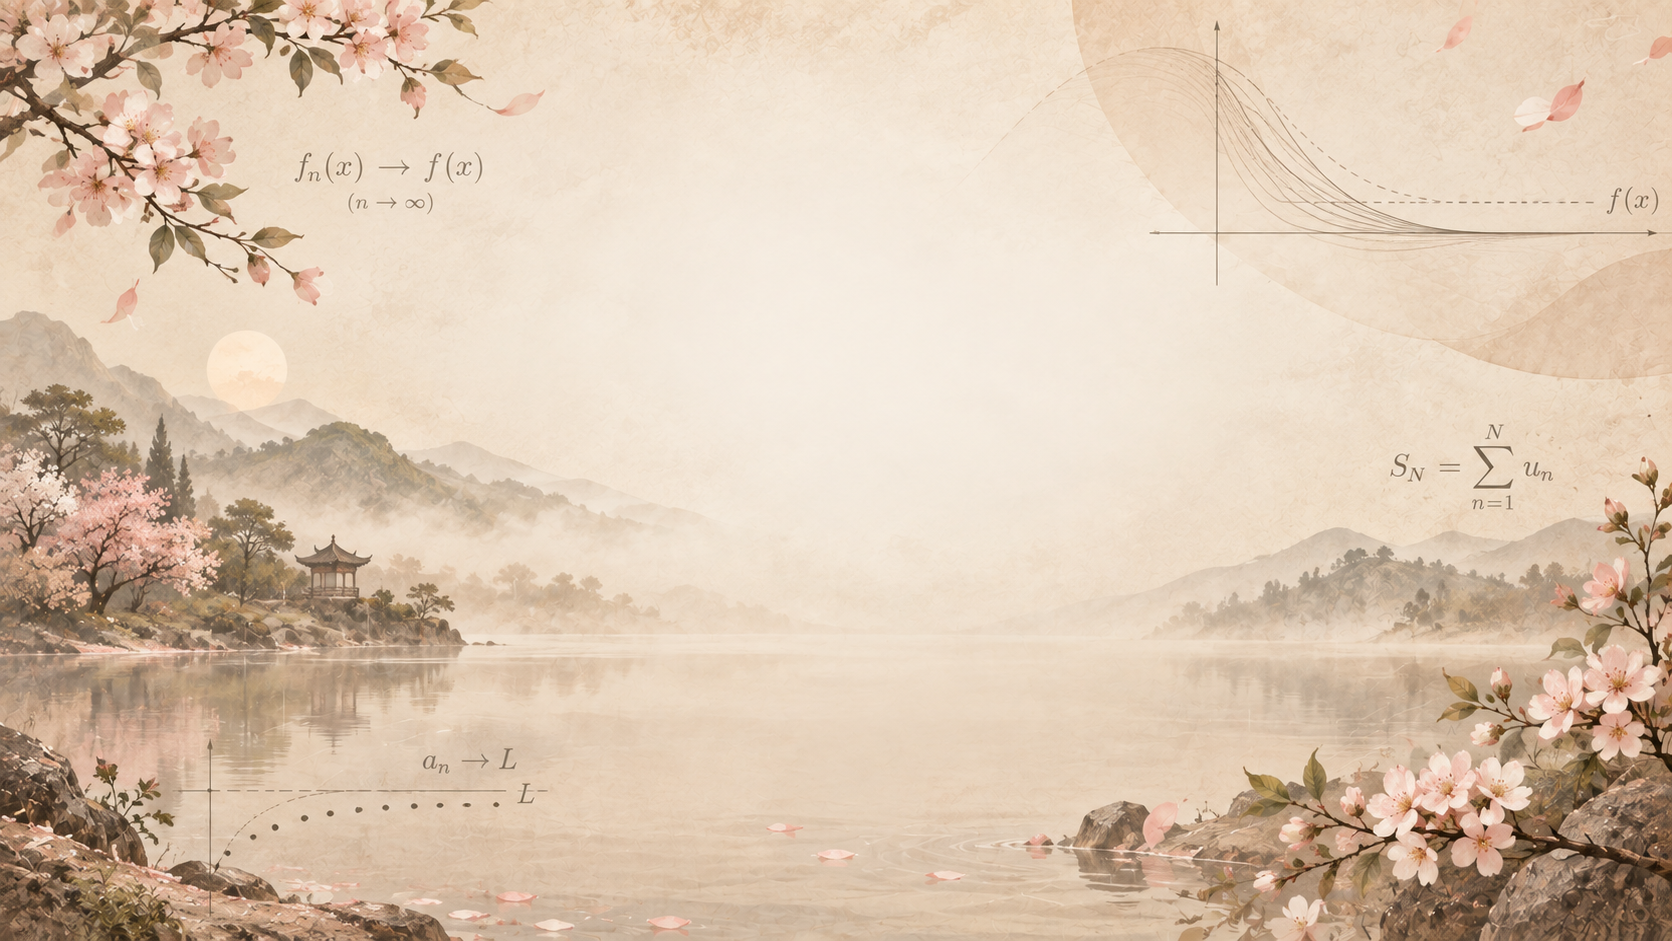
\includegraphics[width=\paperwidth,height=\paperheight,keepaspectratio=false]{chapter_07_bg_05.png}%
}
\section{Remarks}

\begin{frame}{Revisiting Example 7.6}
  \begin{remblock}{Remark: why Theorem 7.16 does not apply}
    For $f_n(x) = n\,x(1-x^2)^n$, the peak is at $x = 1/\sqrt{2n+1}$:
    \[
      \sup_{0 \le x \le 1} |f_n(x) - 0|
      = \frac{n}{\sqrt{2n+1}} \Bigl(1 - \frac{1}{2n+1}\Bigr)^{n}
      \approx \sqrt{\frac{n}{2e}} \;\to\; \infty.
    \]
    So $f_n \to 0$ \alert{not uniformly}. Conversely, Theorem 7.16 alone
    \emph{proves} non-uniformity: $\int_0^1 f_n \to \tfrac12 \ne 0$.
  \end{remblock}

  \note{
    Let's return to Example 7.6 and see why it does not contradict the
    theorem. Setting the derivative of "f" sub "n" to zero, the peak of
    the bump is at "x" equal to 1 over the square root of 2 "n" plus 1.
    The height there is roughly the square root of "n" over 2 "e", which
    grows without bound. These are the tall peaks we saw in the plot. So
    the supremum of the error tends to infinity, and by Theorem 7.9 the
    convergence is not uniform. Notice that we could also argue
    backwards: if the convergence were uniform, Theorem 7.16 would force
    the integrals to tend to zero, but they tend to one half.
  }
\end{frame}

\begin{frame}{Uniform Convergence Is Sufficient, Not Necessary}
  \begin{columns}[T]
    \begin{column}{0.4\textwidth}
      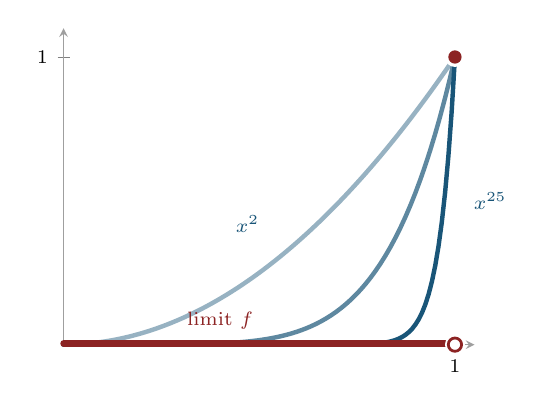
\begin{tikzpicture}
        \begin{axis}[
          axis background/.style={fill=white, fill opacity=0.6},
          width=6.8cm, height=5.6cm,
          xmin=0, xmax=1.05, ymin=0, ymax=1.1,
          axis lines=left, axis line style={gray!75},
          xtick={1}, ytick={1}, clip=false,
          tick label style={font=\scriptsize},
          every axis plot/.append style={curveln},
        ]
          \addplot[domain=0:1, samples=80, defcolor!45] {x^2};
          \addplot[domain=0:1, samples=80, defcolor!70] {x^6};
          \addplot[domain=0:1, samples=120, defcolor] {x^25};
          \addplot[thmcolor, line width=2.4pt] coordinates {(0,0.004) (0.985,0.004)};
          \node[font=\scriptsize, thmcolor, above] at (axis cs:0.4,0.02) {limit $f$};
          \node[font=\scriptsize, defcolor] at (axis cs:0.47,0.42) {$x^2$};
          \node[font=\scriptsize, defcolor] at (axis cs:1.09,0.5) {$x^{25}$};
          \opendotpt{thmcolor}{(axis cs:1,0)}
          \dotpt{thmcolor}{(axis cs:1,1)}
        \end{axis}
      \end{tikzpicture}
    \end{column}
    \begin{column}{0.58\textwidth}
      \begin{remblock}{Remark: the converse fails}
        $f_n(x) = x^n$ on $[0,1]$: the limit $f$ is $0$ on $[0,1)$ and $f(1) = 1$.
        \begin{itemize}
          \item Not uniform (Theorem 7.12: $f$ is discontinuous)
          \item Yet $\displaystyle\int_0^1 x^n\,dx = \frac{1}{n+1} \to 0 = \int_0^1 f\,dx$
        \end{itemize}
      \end{remblock}
    \end{column}
  \end{columns}

  \note{
    The theorem gives a sufficient condition, not a necessary one. In
    the plot on the left, the blue curves are "x" squared, "x" to the
    sixth, and "x" to the 25th power, getting darker as the exponent
    grows. They converge to the red limit "f": zero along the bottom
    edge, shown by the thick red line ending in an open dot at 1, and
    then a jump to the value 1, marked by the filled red dot at the top
    right. The limit is discontinuous, so by Theorem 7.12 the
    convergence cannot be uniform. Nevertheless, the integrals, 1 over
    "n" plus 1, tend to zero, which is the integral of the limit. So
    interchanging limit and integral can work without uniformity; the
    Lebesgue theory of Chapter 11 explains why.
  }
\end{frame}

\begin{frame}{Why the Bounded Interval Matters}
  \begin{columns}[T]
    \begin{column}{0.44\textwidth}
      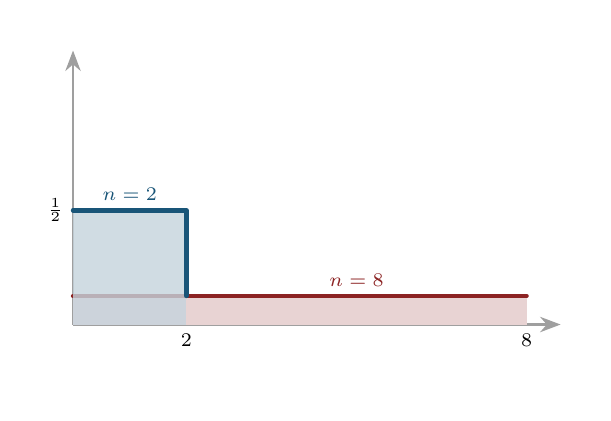
\begin{tikzpicture}[x=0.72cm,y=2.9cm]
        \fill[white, opacity=0.6] (-0.8,-0.3) rectangle (9.0,1.3);
        \draw[axisln] (0,0) -- (8.6,0);
        \draw[axisln] (0,0) -- (0,1.2);
        \fill[thmcolor!20] (0,0) rectangle (8,0.125);
        \draw[thmcolor, curveln] (0,0.125) -- (8,0.125);
        \fill[defcolor!25, opacity=0.8] (0,0) rectangle (2,0.5);
        \draw[defcolor, curveln] (0,0.5) -- (2,0.5) -- (2,0.125);
        \node[font=\scriptsize, defcolor, above] at (1,0.5) {$n = 2$};
        \node[font=\scriptsize, thmcolor, above] at (5,0.125) {$n = 8$};
        \foreach \t in {2,8} \node[below, font=\scriptsize] at (\t,0) {$\t$};
        \node[left, font=\scriptsize] at (0,0.5) {$\tfrac12$};
      \end{tikzpicture}
    \end{column}
    \begin{column}{0.54\textwidth}
      \begin{remblock}{Remark: compact interval}
        \raggedright
        On $[0, \infty)$ let
        $f_n = \tfrac{1}{n}$ on $[0, n]$, $0$ elsewhere.
        \begin{itemize}
          \item $\sup |f_n| = \tfrac1n \to 0$ \ (\alert{uniform})
          \item but $\int_0^\infty f_n\,dx = 1$ for \emph{every} $n$
        \end{itemize}
        (improper integrals; the interval has \alert{infinite} length)
      \end{remblock}
    \end{column}
  \end{columns}

  \note{
    One more remark, beyond the text, shows why the theorem is stated on
    a closed bounded interval. On the half line, let "f" sub "n" equal 1
    over "n" on the interval from zero to "n", and zero beyond. The
    picture shows two of these as flat rectangles: the blue one for "n"
    equal to 2, of height one half and width 2, and the red one for "n"
    equal to 8, lower and wider. The heights tend to zero uniformly, yet
    every rectangle has area 1, so the improper integrals stay at 1. In
    the proof, the factor alpha of "b" minus alpha of "a" in equation 26
    was finite; on an infinite interval it becomes infinite, and the
    error bound no longer goes to zero.
  }
\end{frame}
}

{
\usebackgroundtemplate{%
  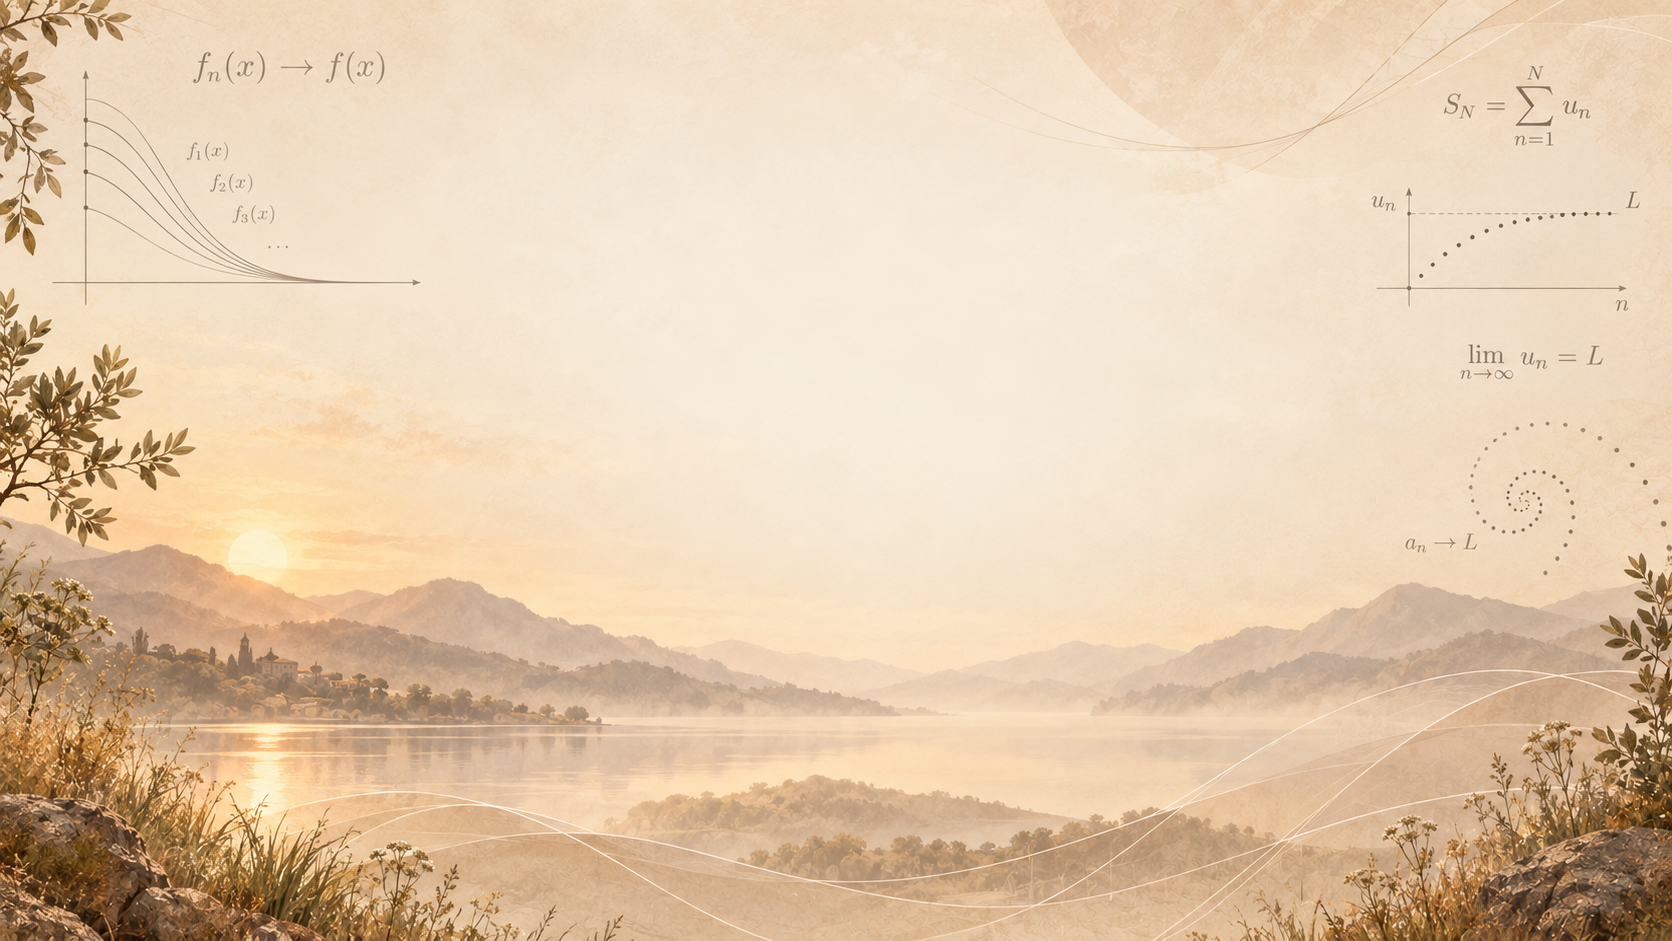
\includegraphics[width=\paperwidth,height=\paperheight,keepaspectratio=false]{chapter_07_bg_06.png}%
}
\section{Summary}

% --- Build 1/3 ---
\begin{frame}{Summary}
  \begin{hlbox}
  \textbf{Key takeaways from this section:}
  \begin{itemize}
    \item \textbf{Theorem 7.16:} $f_n \in \mathscr{R}(\alpha)$, $f_n \to f$
      \alert{uniformly} on $[a,b]$ $\Rightarrow$ $f \in \mathscr{R}(\alpha)$ and
      $\int f\,d\alpha = \lim \int f_n\,d\alpha$
  \end{itemize}
  \end{hlbox}

  \note{
    Let's review. Theorem 7.16 says that if integrable functions
    converge uniformly on a closed interval, then the limit is
    integrable, and the integral of the limit is the limit of the
    integrals. The existence of that limit is part of the conclusion.
  }
\end{frame}

% --- Build 2/3 ---
\begin{frame}{Summary}
  \begin{hlbox}
  \textbf{Key takeaways from this section:}
  \begin{itemize}
    \item \textbf{Theorem 7.16:} $f_n \in \mathscr{R}(\alpha)$, $f_n \to f$
      \alert{uniformly} on $[a,b]$ $\Rightarrow$ $f \in \mathscr{R}(\alpha)$ and
      $\int f\,d\alpha = \lim \int f_n\,d\alpha$
    \item \textbf{Proof:} tube $f_n \pm \varepsilon_n$ squeezes upper and lower
      integrals; \\
      error $\le \varepsilon_n[\alpha(b) - \alpha(a)]$
  \end{itemize}
  \end{hlbox}

  \note{
    The proof was a squeeze. The limit function lies in a tube of half
    width epsilon sub "n" around "f" sub "n". Integrating the tube traps
    the upper and lower integrals of "f" in an interval whose length
    tends to zero, which gives integrability, and the same interval
    bounds the error by epsilon sub "n" times alpha of "b" minus alpha
    of "a".
  }
\end{frame}

% --- Build 3/3 ---
\begin{frame}{Summary}
  \begin{hlbox}
  \textbf{Key takeaways from this section:}
  \begin{itemize}
    \item \textbf{Theorem 7.16:} $f_n \in \mathscr{R}(\alpha)$, $f_n \to f$
      \alert{uniformly} on $[a,b]$ $\Rightarrow$ $f \in \mathscr{R}(\alpha)$ and
      $\int f\,d\alpha = \lim \int f_n\,d\alpha$
    \item \textbf{Proof:} tube $f_n \pm \varepsilon_n$ squeezes upper and lower
      integrals; \\
      error $\le \varepsilon_n[\alpha(b) - \alpha(a)]$
    \item \textbf{Corollary:} uniformly conv. series can be
      \alert{integrated term by term}
  \end{itemize}

  \vspace{0.4em}
  \textbf{Coming up next:} uniform convergence and \alert{differentiation}.
  \end{hlbox}

  \note{
    The corollary lets us integrate uniformly convergent series term by
    term, as we did with the geometric series. We also saw that
    uniformity is sufficient but not necessary, and that the bounded
    interval matters. In the next section, Uniform Convergence and
    Differentiation, we face the hardest case of the main problem.
    There, uniform convergence of the functions is not enough, and we
    will need uniform convergence of the derivatives instead. See you
    next time.
  }
\end{frame}
}

\end{document}
